\section{Testi}

\begin{frame}{Stringhe}
	\begin{block}{Chiameremo stringhe..}
        \begin{itemize}
            \item Testi
            \item Insieme di caratteri della tastiera
            
            ! qualsiasi carattere (lettere, numeri, punti, virgole, simboli ecc..)
        \end{itemize}

        \begin{figure}
            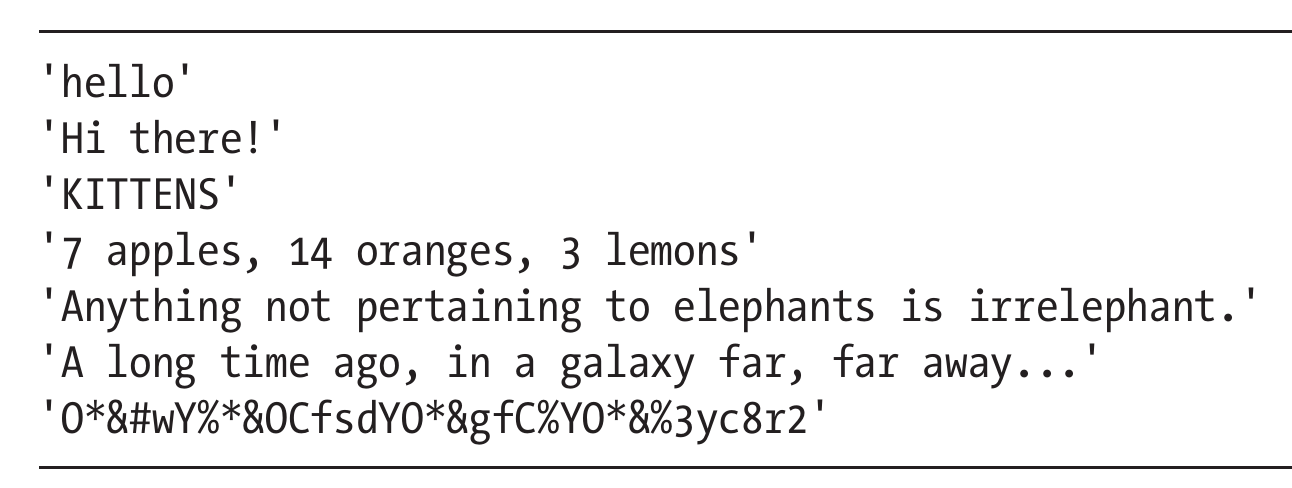
\includegraphics[height=3cm]{images/esempio_stringhe.png}
        \end{figure}
	\end{block}
	
	Notiamo negli esempi l'uso degli apici, all'interno dei quali viene scritta la stringa.
\end{frame}

\begin{frame}{Stringhe}
	\begin{block}{' ' oppure " " ?}
        \begin{itemize}
            \item Entrambi dicono a Python quando inizia e quando finisce una stringa
            \item Non ci sono particolari differenze, possiamo usarli come preferiamo.
            
            Ricordiamoci però di usare sempre lo stesso simbolo per l'inizio e la fine della stringa.
            
            'Ciao' OK
            
            \textbf{'}Ciao\textbf{"} NO
        \end{itemize}
	\end{block}
\end{frame}

\begin{frame}{Possiamo \textbf{concatenare} stringhe}
    \begin{itemize}
        \item 'Ciao ' + ' Ragazze Digitali'
        \item nome = 'Enrico'
            
        'Ciao ' + nome
        \item Ma non solo..
    \end{itemize}

	\begin{block}{Cosa succede se..}
        \begin{itemize}
            \item nome = Enrico
            
            \lstinline{NameError: name 'Enrico' is not defined}
            
            (Si aspetta una variabile di nome Enrico che non esiste, questo perchè non ho messo gli 'apici')
            \item 'Oggi siete in ' + numeroRagazzeSummerCamp
            
            \lstinline{TypeError: cannot concatenate 'str' and 'int' objects}
            
            Non posso concatenare stringhe con numeri, posso però convertire numeroRagazzeSummerCamp in stringa, vedremo come
        \end{itemize}
    \end{block}
\end{frame}